%#!latex
%\documentclass[luatex]{nolta}
%\documentclass[xetex]{nolta}
\documentclass[dvipdfmx]{nolta}
%\documentclass[pdftex,survey]{nolta}

% \documentclass[pdftex]{nolta}


\newcommand{\NOLTA}{\textbf{NOLTA}}


\Vol{2}%
\No{3}%
\Year{2011}%
\Month{10}%

%
%\printorcid
%

\setcounter{page}{1101}%%

\title{Instructions/template for preparing
your NOLTA manuscript\\
\textcolor{red}{(Ver.\ 5.1, December 17, 2024)}}

\AUTHOR*{%
\author{Name Author1}{1}\orcid{000-0000-0000-0000},
\author*{Name Author2}{2}\orcid{000-0000-0000-0000},
\author{Name Author3}{1}\orcid{000-0000-0000-0000}
}


\AFFILIATE{%
\affiliate{Institute of Industrial Science, University of XXXXX\\
1-2-3 Address, City 000-0000, Country}{1},
\affiliate{Electrical and Electronics Lab, XXXX Laboratories Co. \\
3-2-1 Address, City 000-0000, Country}{2}
}



\received{10}{27}{20XX}
\revised{12}{29}{20XX}
\published{7}{1}{20XX}

\begin{document}

\begin{abstract}
Use this instruction file as a template for preparing your {\NOLTA}
articles with \LaTeX.  It is essential to adhere to this template
because final post-peer review manuscripts are published as is, with
minimal editing/formatting by the publisher.  Do not modify any formats
or styles.
Visit Information for Authors
\url{https://www.ieice.org/nolta/journal/author.html} for the
latest version of {\NOLTA} template.
\end{abstract}

\begin{keywords}
NOLTA, template, nolta.cls, up to six words
\end{keywords}

\maketitle

\section{Introduction}
Deep learning has achieved remarkable success in various fields, such as image recognition and natural language processing. The generalization performance of deep neural networks has often been improved by increasing model size, the amount of training data, and computational resources. This tendency is often characterized by scaling laws, which describe how model performance improves as these resources are scaled up.

However, such resource-based scaling is not always applicable in practical situations. In some domains, such as industrial anomaly detection and medical applications, it is difficult to collect a large amount of labeled data, especially for rare or abnormal cases. In addition, some applications must be performed under limited computational resources, memory capacity, or inference time. Therefore, it is important to explore alternative learning paradigms that can improve generalization performance without simply relying on larger models, larger datasets, or larger computational budgets.

In recent years, collaborative learning frameworks using multiple models have attracted attention as one possible approach. These frameworks use the predictions of other models as additional supervision during training, thereby improving generalization performance. Since model collaboration is required only during training, these frameworks can improve model performance without increasing the computational cost at inference time.

A representative example of such frameworks is Mutual learning (ML), in which multiple models are trained simultaneously while referring to each other's prediction distributions. Unlike conventional teacher-student approaches, ML does not require a fixed pre-trained teacher model. In ML, each model is trained using a loss function consisting of a standard supervised loss and a KL-divergence-based consistency loss between prediction distributions. Previous studies have shown that ML often achieves better generalization performance than independently trained models. However, it remains unclear how ML improves model performance, particularly how interactions between models during training contribute to this improvement.

In this study, the generalization process of ML is analyzed by comparing ML models with individual learning (IL) models. The double descent phenomenon is used as the main analytical framework because it contradicts the conventional bias-variance trade-off and involves non-monotonic changes in test error, which can reveal characteristics of the generalization process. First, differences in double descent behavior between ML and IL are examined with respect to the number of model parameters and training epochs. As further analyses, ML and IL are compared in terms of variance, loss landscape geometry, and Hessian-based properties, especially across the regimes of double descent. Their convergence behavior on clean and noisy data is also analyzed to examine how ML affects robustness to label noise.

The main contributions of this study are summarized as follows:
\begin{itemize}
\item The analysis suggests that ML and IL can differ in aspects that are not apparent from test performance alone.

\item The results show that the effect of ML is regime-dependent. In particular, around the Critical Regime, ML tends to suppress overfitting, delay fitting to noisy labels, and reduce the increase in variance.

\item The analysis provides evidence that ML and IL differ in aspects that are not captured by test performance alone. Even when their final test errors are comparable in the Over-parameterized Regime, ML and IL show different tendencies in the loss landscape geometry and the top eigenvalues of the Hessian.

\end{itemize}

\section{Related Works}
\subsection{Mutual Learning}

Mutual learning is a training framework in which multiple models are trained simultaneously by referring to each other's predictions. In individual learning, each model is optimized independently using only the ground-truth labels. In contrast, mutual learning introduces interactions among models during training through their prediction distributions.

In ML, the loss function of each model includes both a supervised loss and a mimicry loss. For two models, let $p_1$ and $p_2$ denote the prediction distributions of Model 1 and Model 2, respectively.
The objective function of each model consists of a cross-entropy loss and a Kullback--Leibler (KL) divergence term:
\begin{equation}
L_{\Theta_1} = L_{\mathrm{CE}}(y, p_1) + D_{\mathrm{KL}}(p_2 \| p_1),
\end{equation}
\begin{equation}
L_{\Theta_2} = L_{\mathrm{CE}}(y, p_2) + D_{\mathrm{KL}}(p_1 \| p_2).
\end{equation}
The cross-entropy term supervises each model using the ground-truth label $y$, while the KL divergence term encourages the prediction distribution of each model to approach that of the other model.

ML improves generalization performance compared with individual learning across various network architectures and tasks, such as image recognition and person re-identification.
Compact models also benefit from mutual learning without using a large pre-trained teacher model.
Since each model is trained collaboratively but used independently at inference time, ML can improve the training process without increasing the inference cost of a single model.

The effectiveness of ML has been discussed in terms of posterior entropy and robust minima.
Because models are initialized differently, their secondary class probabilities can differ even when they predict the same ground-truth class.
Matching these prediction distributions increases posterior entropy and may guide models toward flatter minima with better generalization.
However, the relationship between mutual learning and the generalization process under changes in model complexity and training time has not been fully characterized.

\subsection{Double Descent}
Double descent is a phenomenon in which the test error first decreases, then increases, and finally decreases again as model complexity increases. This behavior differs from the conventional U-shaped generalization curve expected from the classical bias-variance trade-off. Figure X illustrates a typical double descent curve, where the training error continues to decrease while the test error exhibits a non-monotonic pattern. Depending on the source of complexity, double descent can be categorized into parameter-wise and epoch-wise double descent. Parameter-wise double descent occurs as the number of model parameters increases, whereas epoch-wise double descent occurs as the number of training epochs increases.

\begin{figure}[htb]
  \centering
  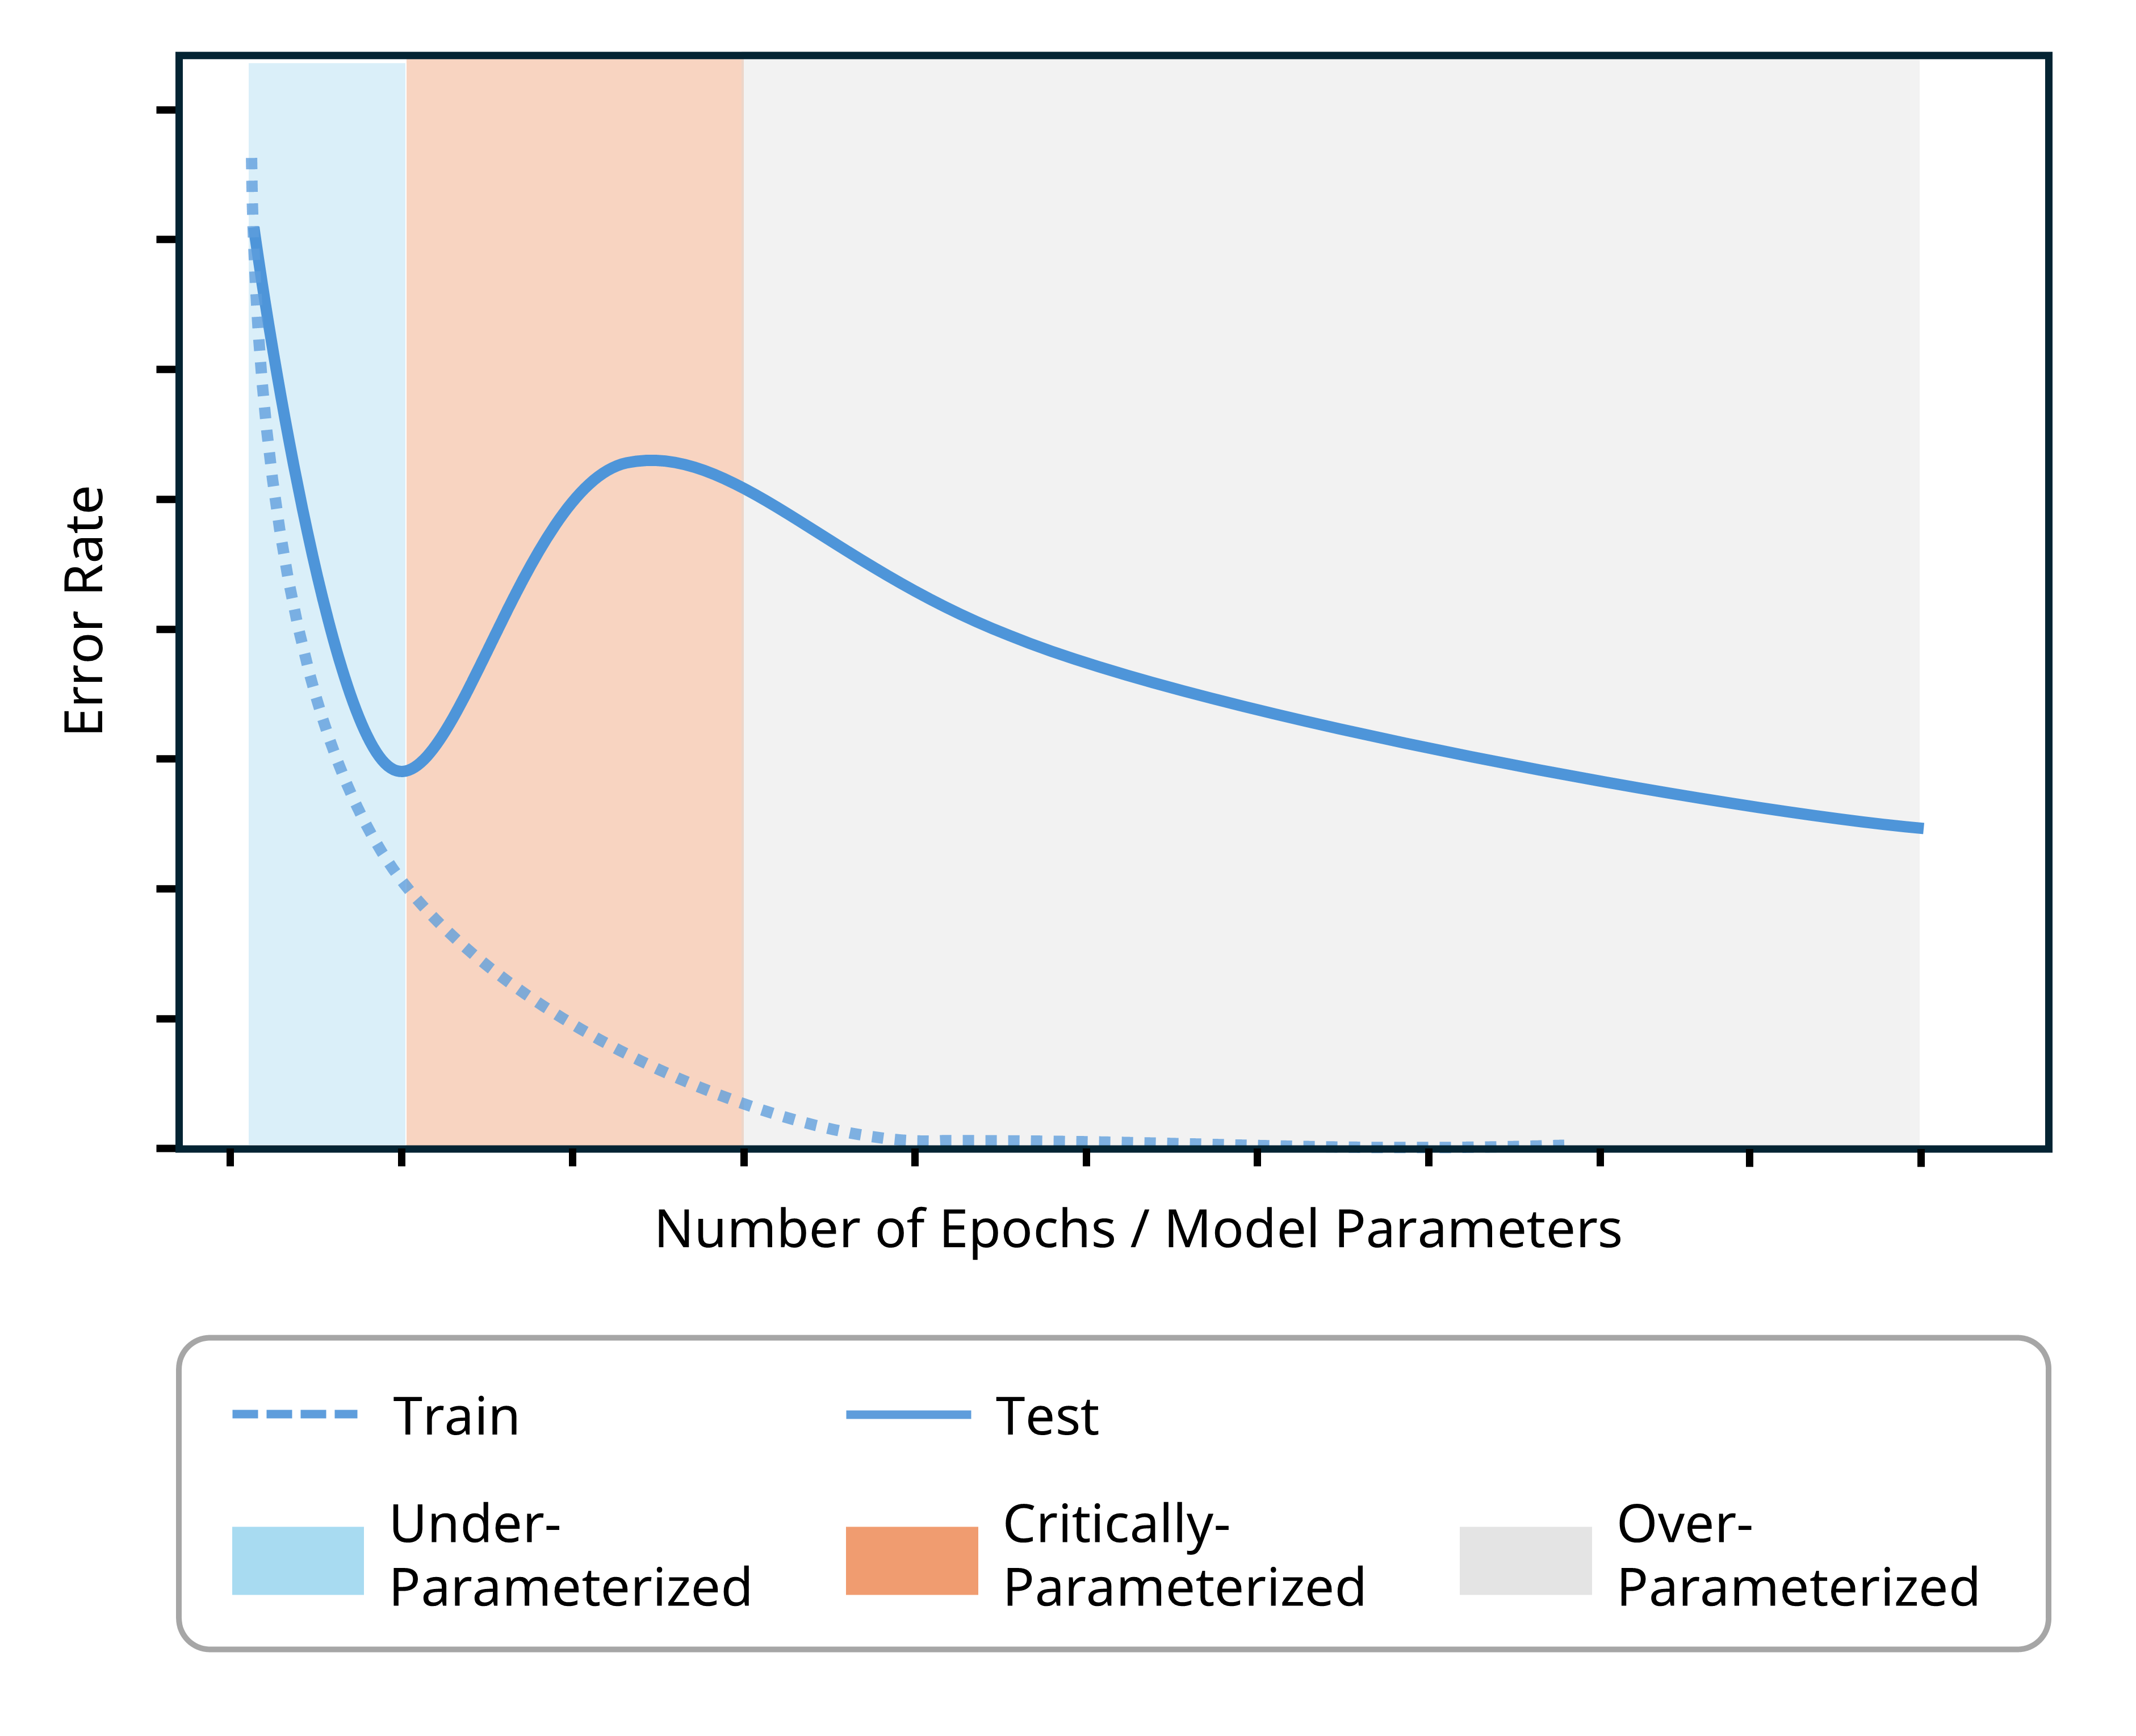
\includegraphics[width=0.8\linewidth]{fig/1_double_descent.png}
  \caption{Caption text.}
  \label{fig:doubledescent}
\end{figure}

The curve is often interpreted by dividing the learning process into three regimes, as shown by the shaded regions in Fig.~\ref{fig:doubledescent}: the under-parameterized regime, the critically-parameterized regime, and the over-parameterized regime, shown in purple, orange, and green, respectively. In the under-parameterized regime, the model does not have sufficient capacity to fit the training data, and increasing model complexity tends to reduce the test error. The critically-parameterized regime appears around the interpolation threshold, where the model starts to fit the training data almost perfectly. In this regime, the test error often increases and forms a local maximum, referred to as the peak of double descent. In the over-parameterized regime, the model has sufficient capacity to fit the training data, and further increasing model complexity tends to reduce the test error again.

Previous studies have also investigated factors that affect the peak of double descent. Label noise tends to make the peak more prominent and thus makes the double descent behavior more clearly observable. Data augmentation shifts the peak toward larger models and reduces its height. Ensemble methods have also been reported to reduce the peak.

\section{Experiments}
We first analyze model-wise and epoch-wise double descent by varying the base number of filters and training epochs, respectively. We then conduct additional analyses related to the underlying generalization mechanism: bias--variance decomposition, loss landscape geometry, the top five eigenvalues of the Hessian matrix, and the behavior on clean and noisy test data.

\subsection{Experimental Setup}

We evaluate ML and IL on an image classification task using CIFAR-10.

CIFAR-10 consists of 50,000 training images and 10,000 test images from 10 classes.
We add 20\% label noise to the training labels.

For both ML and IL, we use a 5-layer CNN consisting of four convolutional layers and one fully connected layer.
The numbers of filters in the four convolutional layers are set to $[k, 2k, 4k, 8k]$, where $k$ denotes the base number of filters.

In ML, two models with different initial weights are trained mutually.
In IL, a single model initialized with the same initial weights as Model 1 in ML is trained individually.
For ML, we report the result of Model 1.
Each result is averaged over five independent runs with different initial weights.

In ML, two models, denoted by $M_1$ and $M_2$, are trained mutually.
The two models are initialized with different initial weights.
In IL, a single model initialized with the same initial weights as $M_1$ is trained individually.
For a fair comparison, we report the results of $M_1$ for ML and compare them with those of the corresponding IL model.

The loss function for IL is the cross-entropy loss.
For ML, the loss function consists of the cross-entropy loss and the KL divergence between the prediction distributions of the two models.
All models are trained for 500 epochs using SGD without momentum.
The batch size is 128, and the learning rate is set to $1/\sqrt{1+t/512}$, where $t$ denotes the training step.

\subsection{Filter-wise Double Descent}
This experiment analyzes how ML and IL behave as the model width increases.
In particular, we investigate whether filter-wise double descent occurs in both methods and how the error curves differ between them.

The base number of filters $k$ is varied from 1 to 60. For each value of $k$, we train the models for 500 epochs and evaluate the training and test error rates.

\begin{figure}[htb]
  \centering
  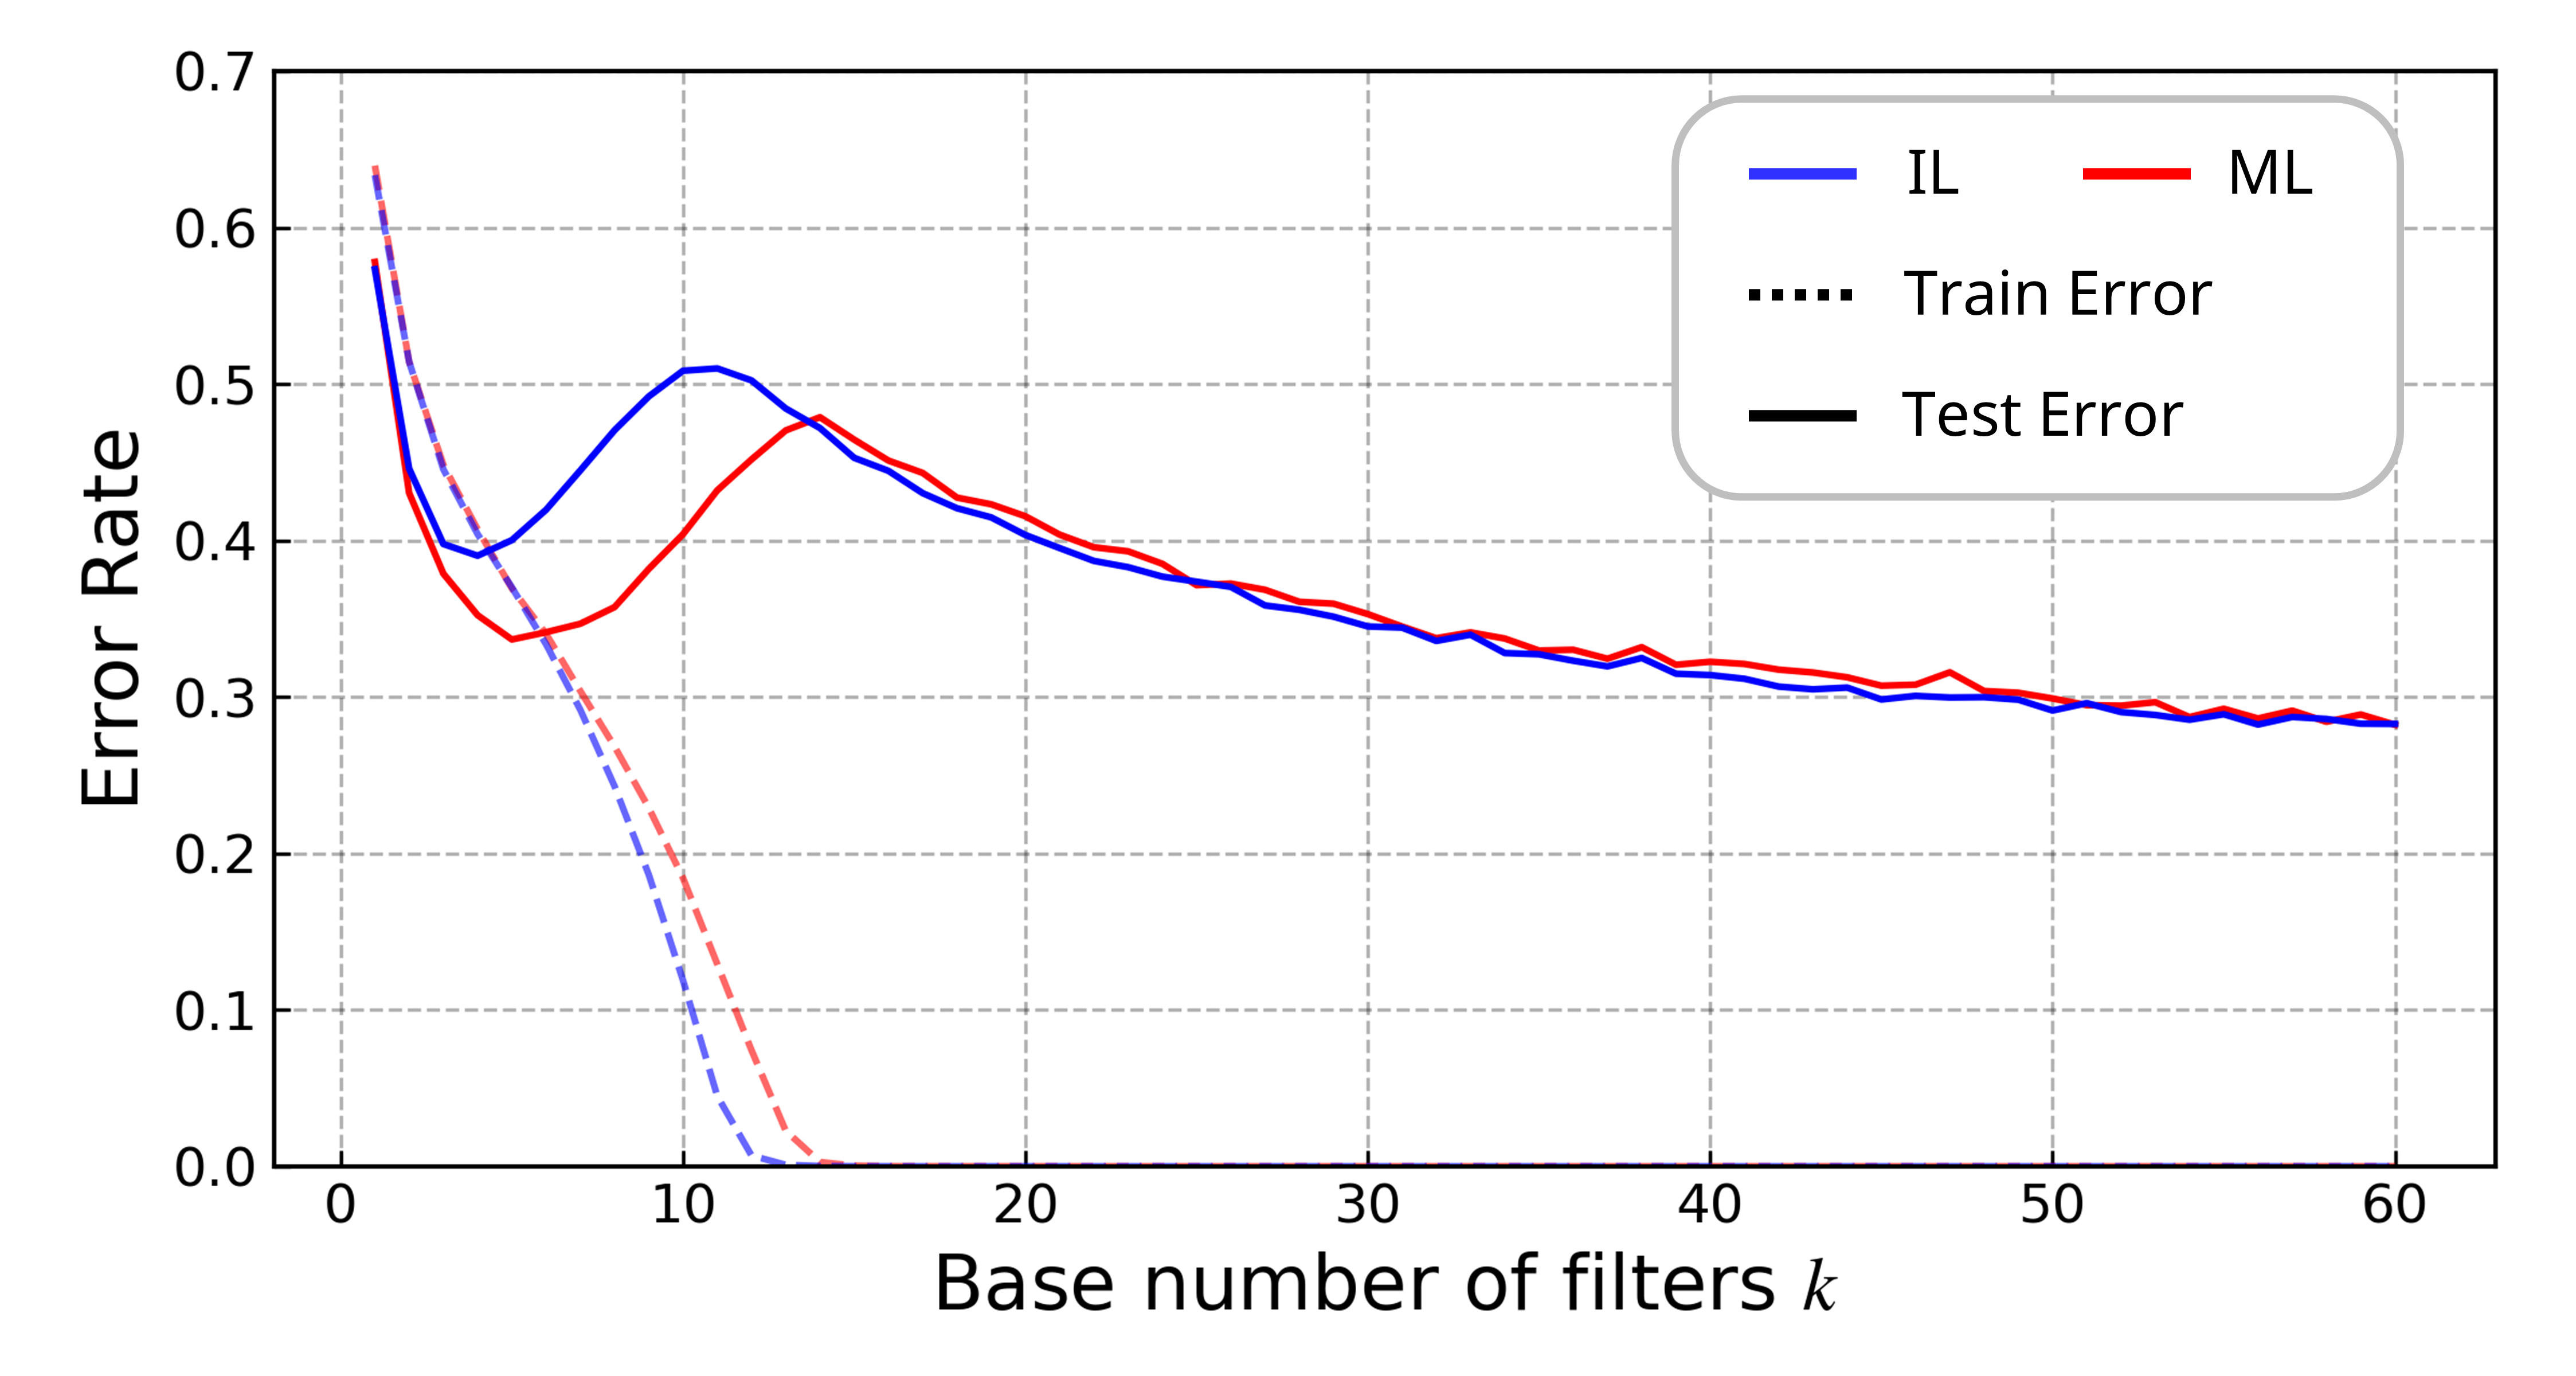
\includegraphics[width=0.8\linewidth]{fig/3_filter_wise.png}
  \caption{Filter-wise double descent of IL and ML as the base number of filters $k$ is varied from 1 to 60.}
  \label{fig:filter_wise}
\end{figure}

Figure~\ref{fig:filter_wise} shows the training and test error rates as functions of the base number of filters $k$.
The blue and red curves represent IL and ML, respectively, while the solid and dashed lines represent the test and training error rates, respectively.

As shown in Figure~\ref{fig:filter_wise}, both IL and ML exhibit filter-wise double descent.
Compared with IL, ML suppresses the test-error peak and shifts the peak position toward larger values of $k$.

To further analyze this difference, we divide the learning behavior into three regimes: the under-parameterized, critically-parameterized, and over-parameterized regimes.

\begin{figure}[htb]
  \centering
  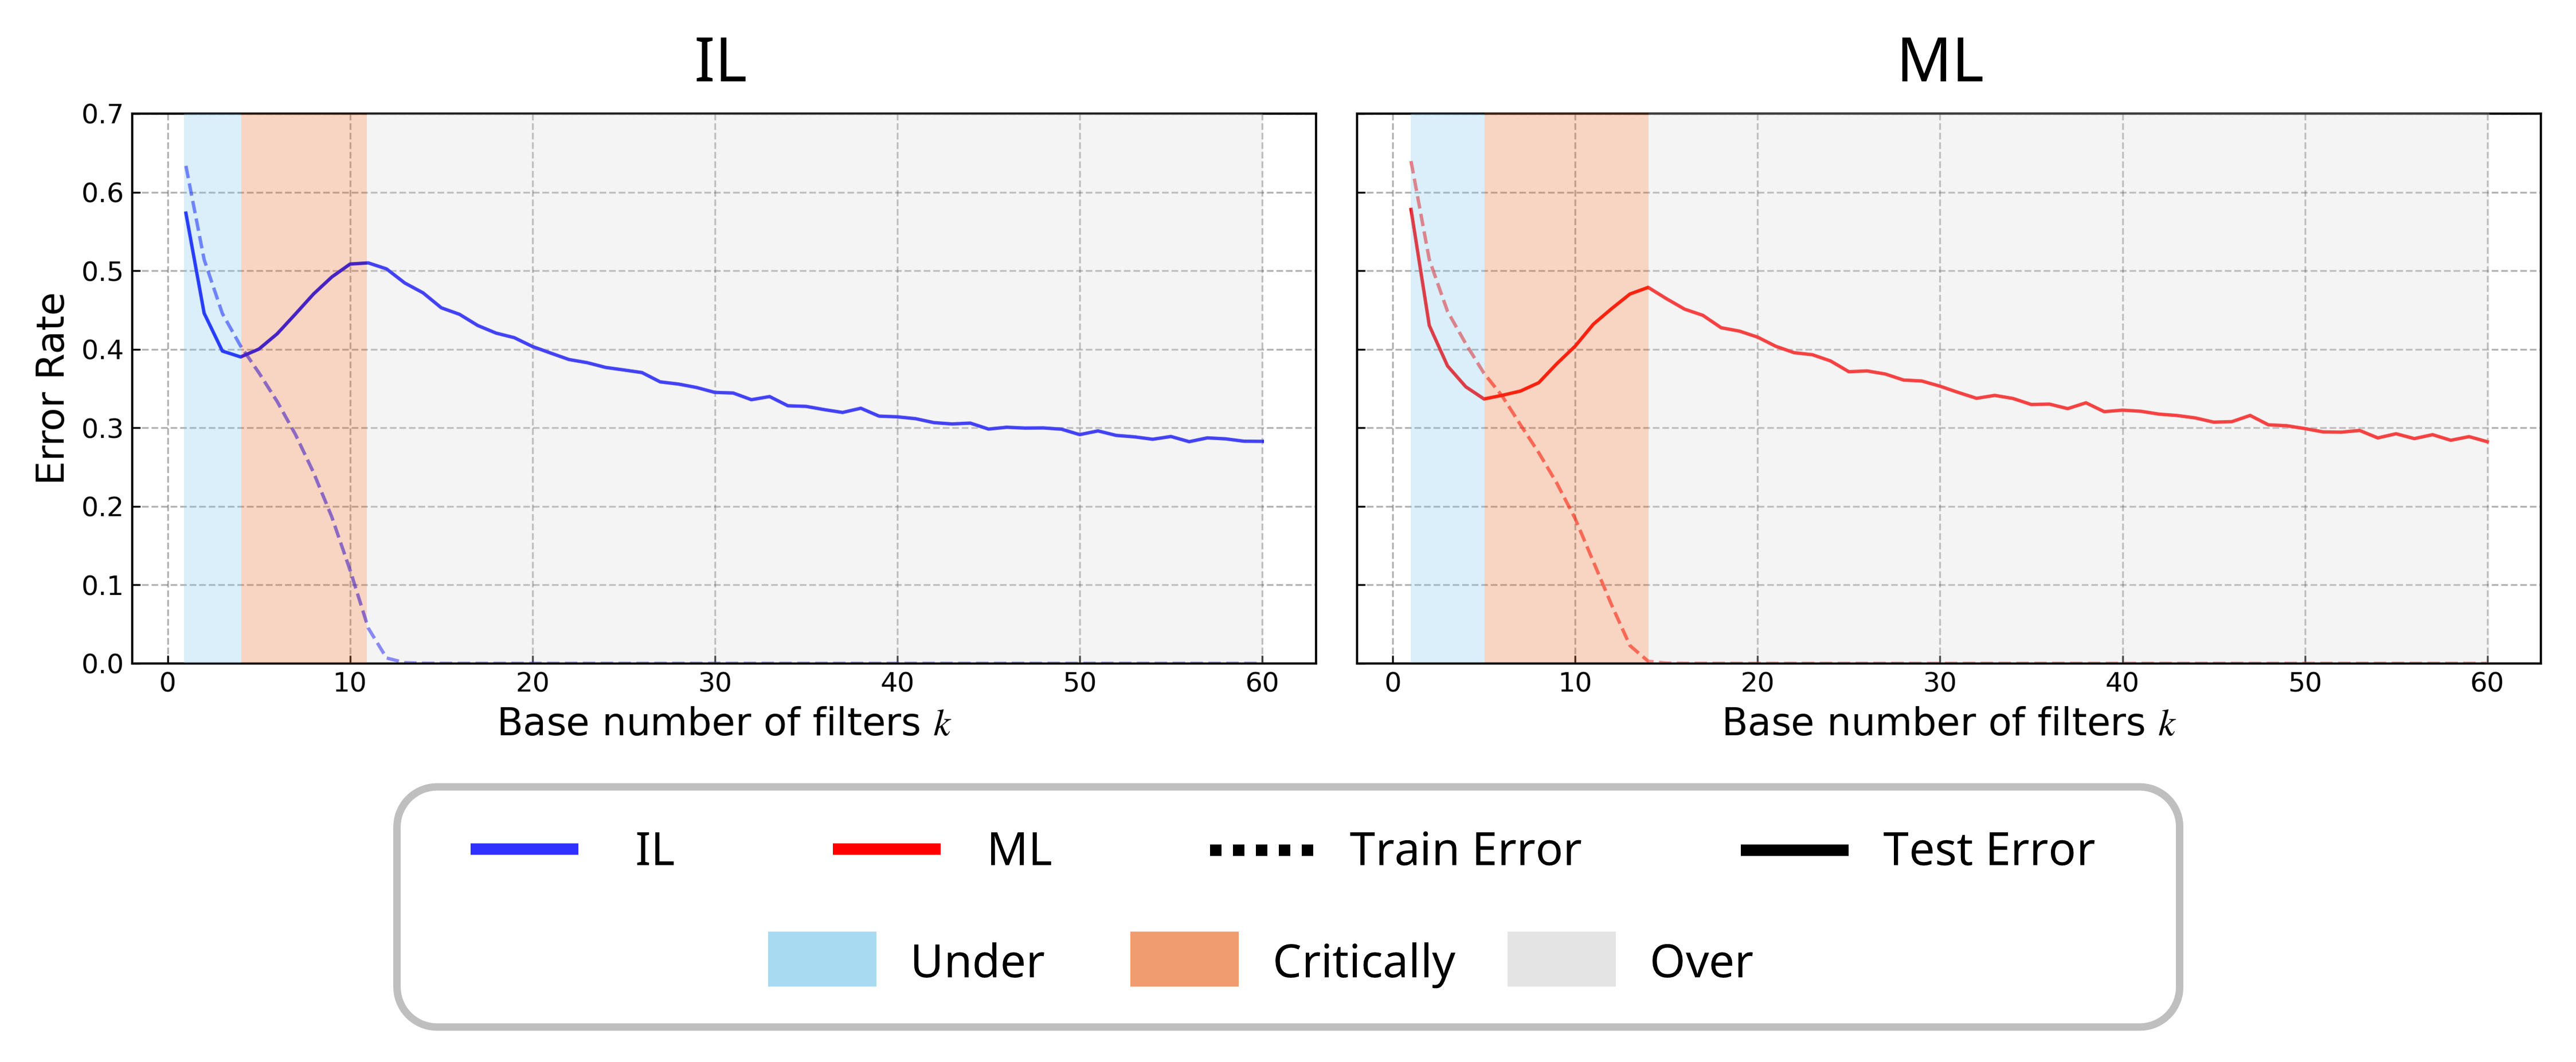
\includegraphics[width=0.8\linewidth]{fig/4_filterwise_regime.png}
  \caption{Regime-wise comparison of filter-wise double descent in IL and ML, where the shaded regions indicate the three regimes.}
  \label{fig:filterwise_regime}
\end{figure}

Figure~\ref{fig:filterwise_regime} visually summarizes the regime transitions of IL and ML.
From this comparison, we observe that the under-parameterized regime is longer in ML than in IL.
The critically-parameterized regime also starts later and lasts longer in ML.
Consequently, the transition to the over-parameterized regime is delayed in ML.

\subsection{Epoch-wise Double Descent}
This experiment analyzes epoch-wise double descent over different model widths.
Specifically, we examine how the error rates of ML and IL change during training for each value of the base number of filters $k$.

\begin{figure}[htb]
  \centering
  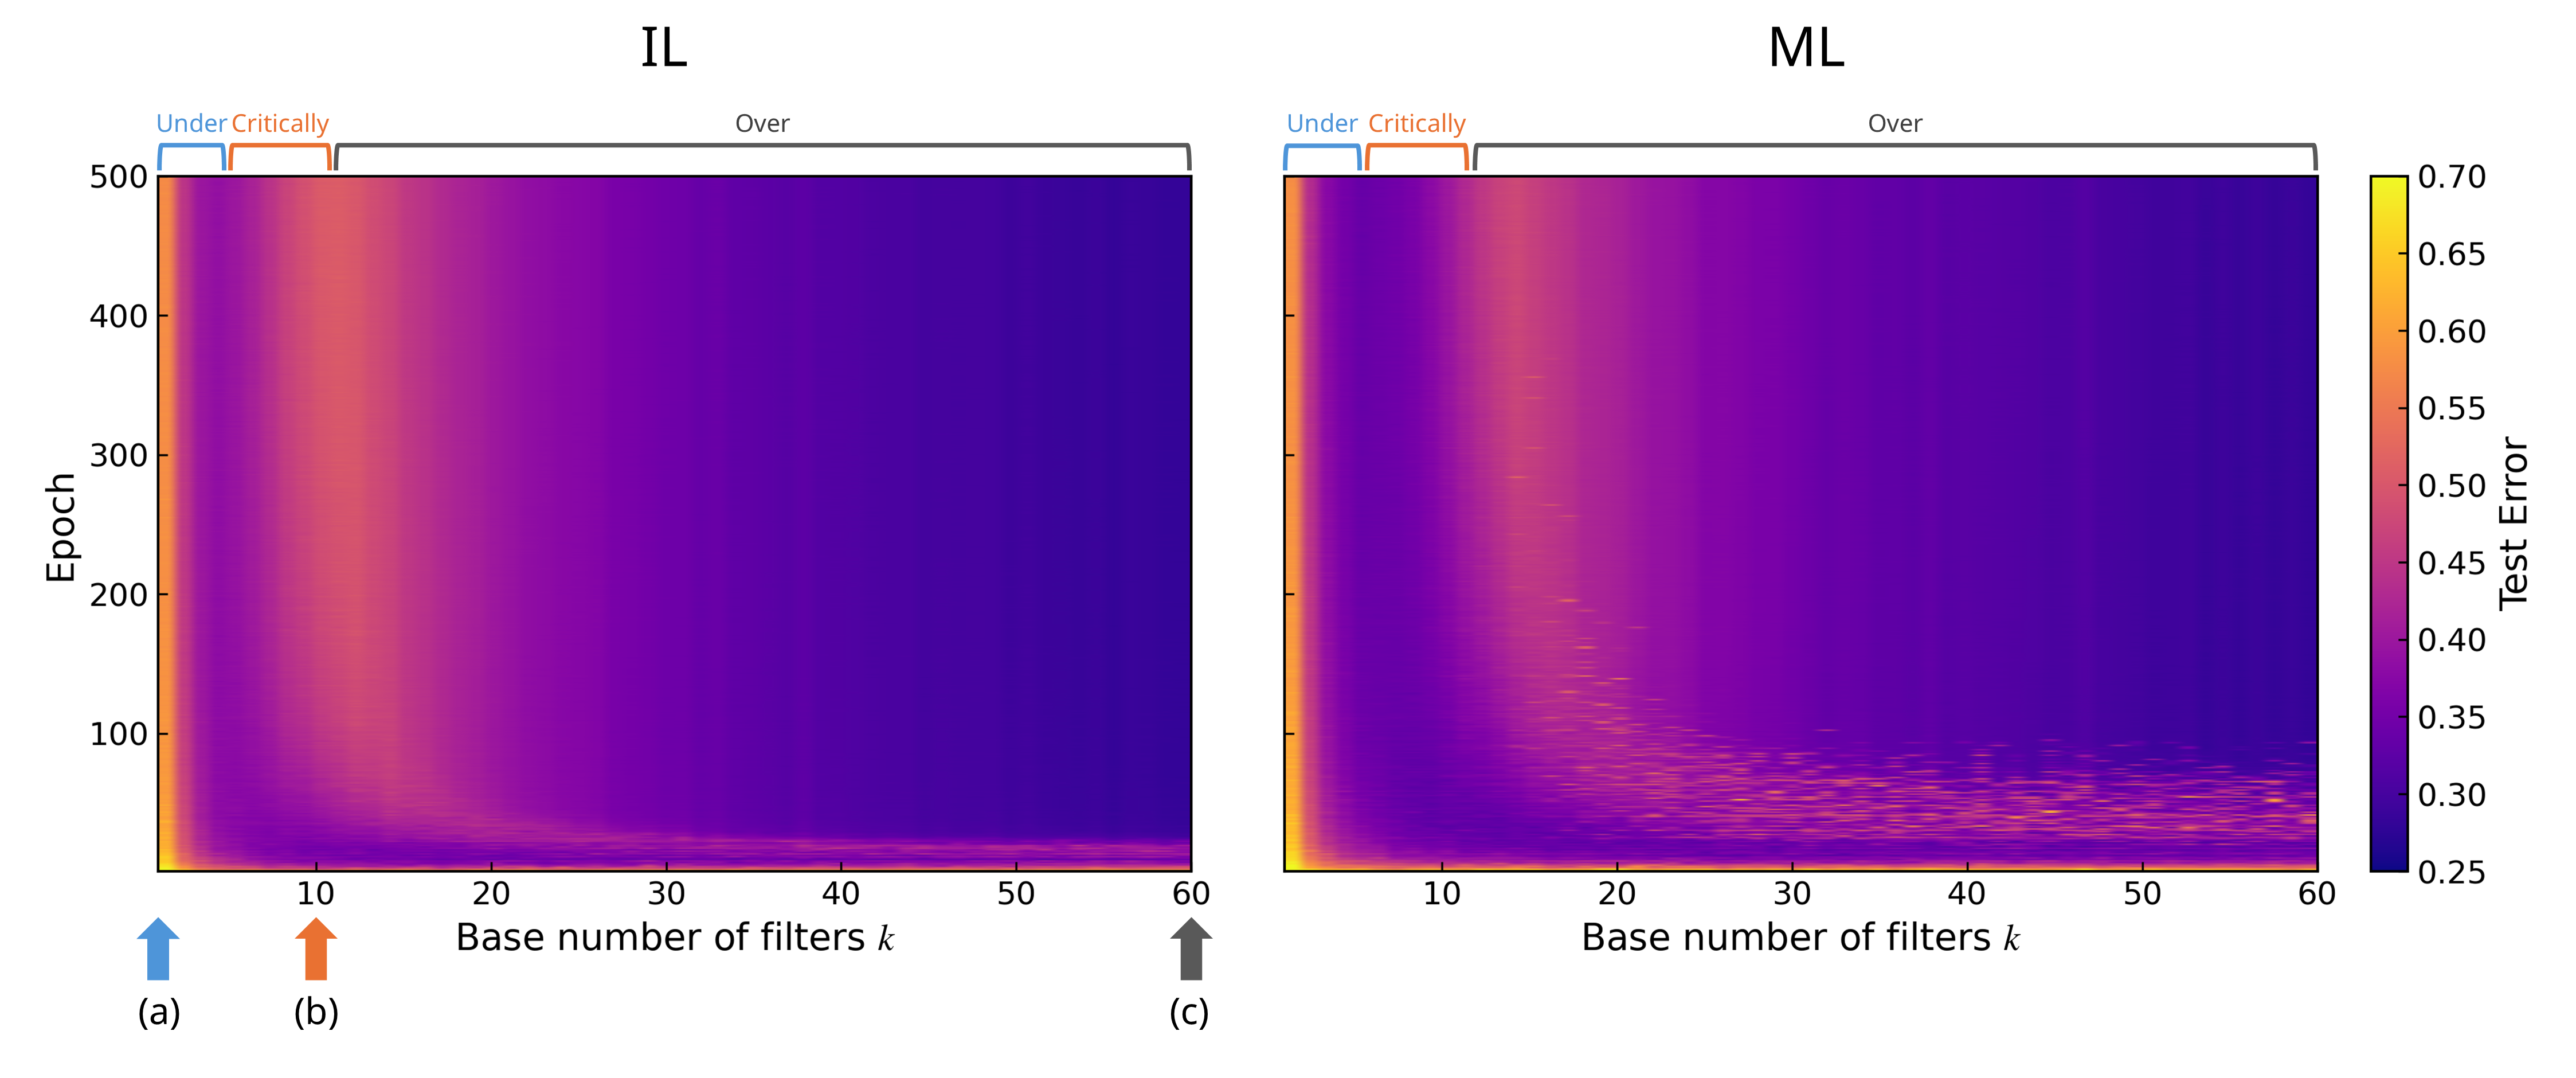
\includegraphics[width=0.8\linewidth]{fig/5_epoch_heatmap_test.png}
  \caption{}
  \label{fig:epoch_heatmap}
\end{figure}

Figure~\ref{fig:epoch_heatmap} shows the test error heatmaps of ML and IL.
The horizontal axis represents the base number of filters $k$, the vertical axis represents the training epoch, and the color represents the test error rate.
The brackets above the heatmaps indicate the regimes identified from the filter-wise double descent results.

As shown in Fig.~\ref{fig:epoch_heatmap}, both ML and IL exhibit regime-dependent epoch-wise behavior.
In the under-parameterized regime, the test error generally decreases as training proceeds.
In the critically-parameterized regime, the test error increases during training, indicating overfitting.
In the over-parameterized regime, the test error shows epoch-wise double descent.
These results indicate that the epoch-wise behavior differs across the regimes in both ML and IL.

\begin{figure}[htb]
  \centering
  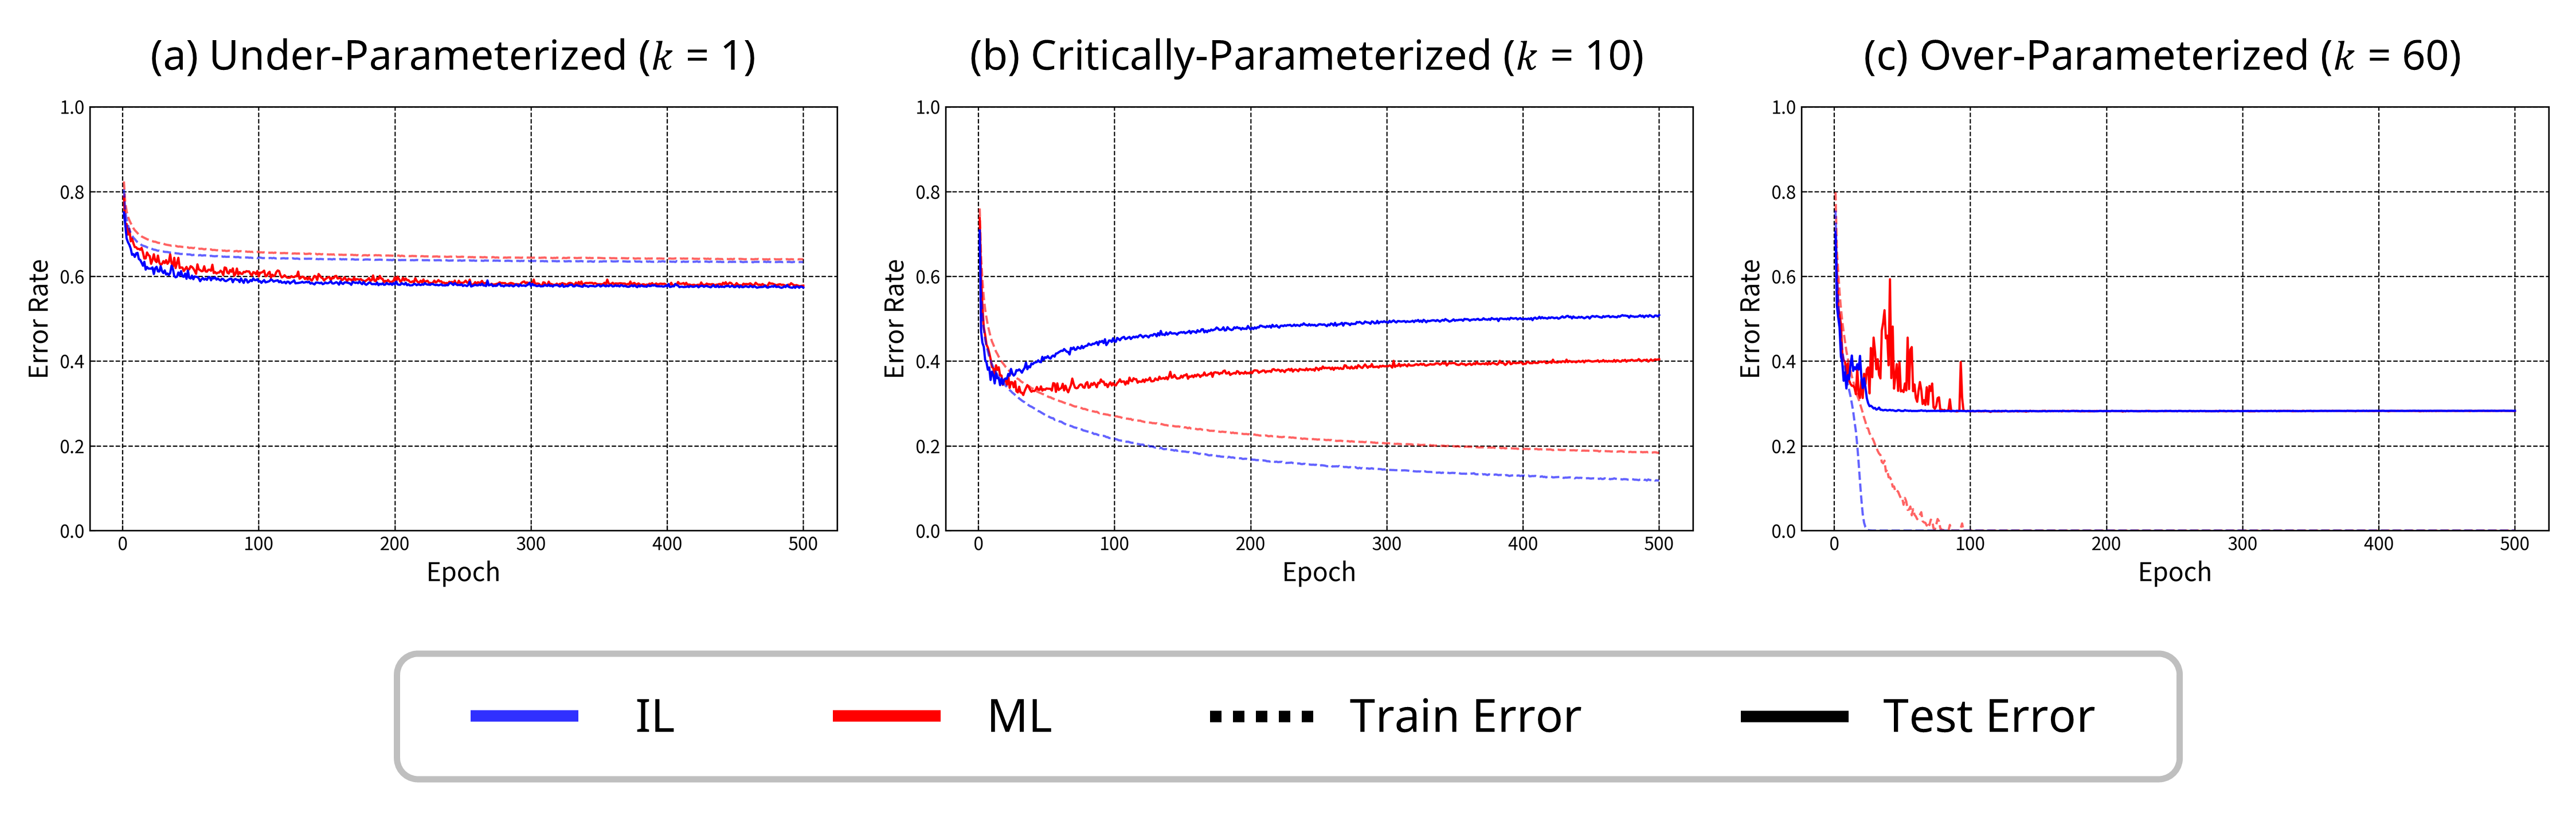
\includegraphics[width=0.8\linewidth]{fig/7_epoch_curves.png}
  \caption{}
  \label{fig:epoch_curves}
\end{figure}

Figure~\ref{fig:epoch_curves} shows representative training and test error curves for selected widths in each regime.
Figures~\ref{fig:epoch_curves} (a), (b), and (c) correspond to the under-parameterized, critically-parameterized, and over-parameterized regimes, respectively.
The solid and dashed lines represent the test and training error rates, respectively.

In the under-parameterized regime, ML and IL show similar test error curves.
In the critically-parameterized regime, ML shows a smaller increase in test error than IL, although its training error decreases more slowly.
In the over-parameterized regime, ML exhibits larger fluctuations in both training and test error, whereas the final test error becomes comparable to that of IL.
These results suggest that the effect of ML is most pronounced around the critically-parameterized regime.

\begin{figure}[htb]
  \centering
  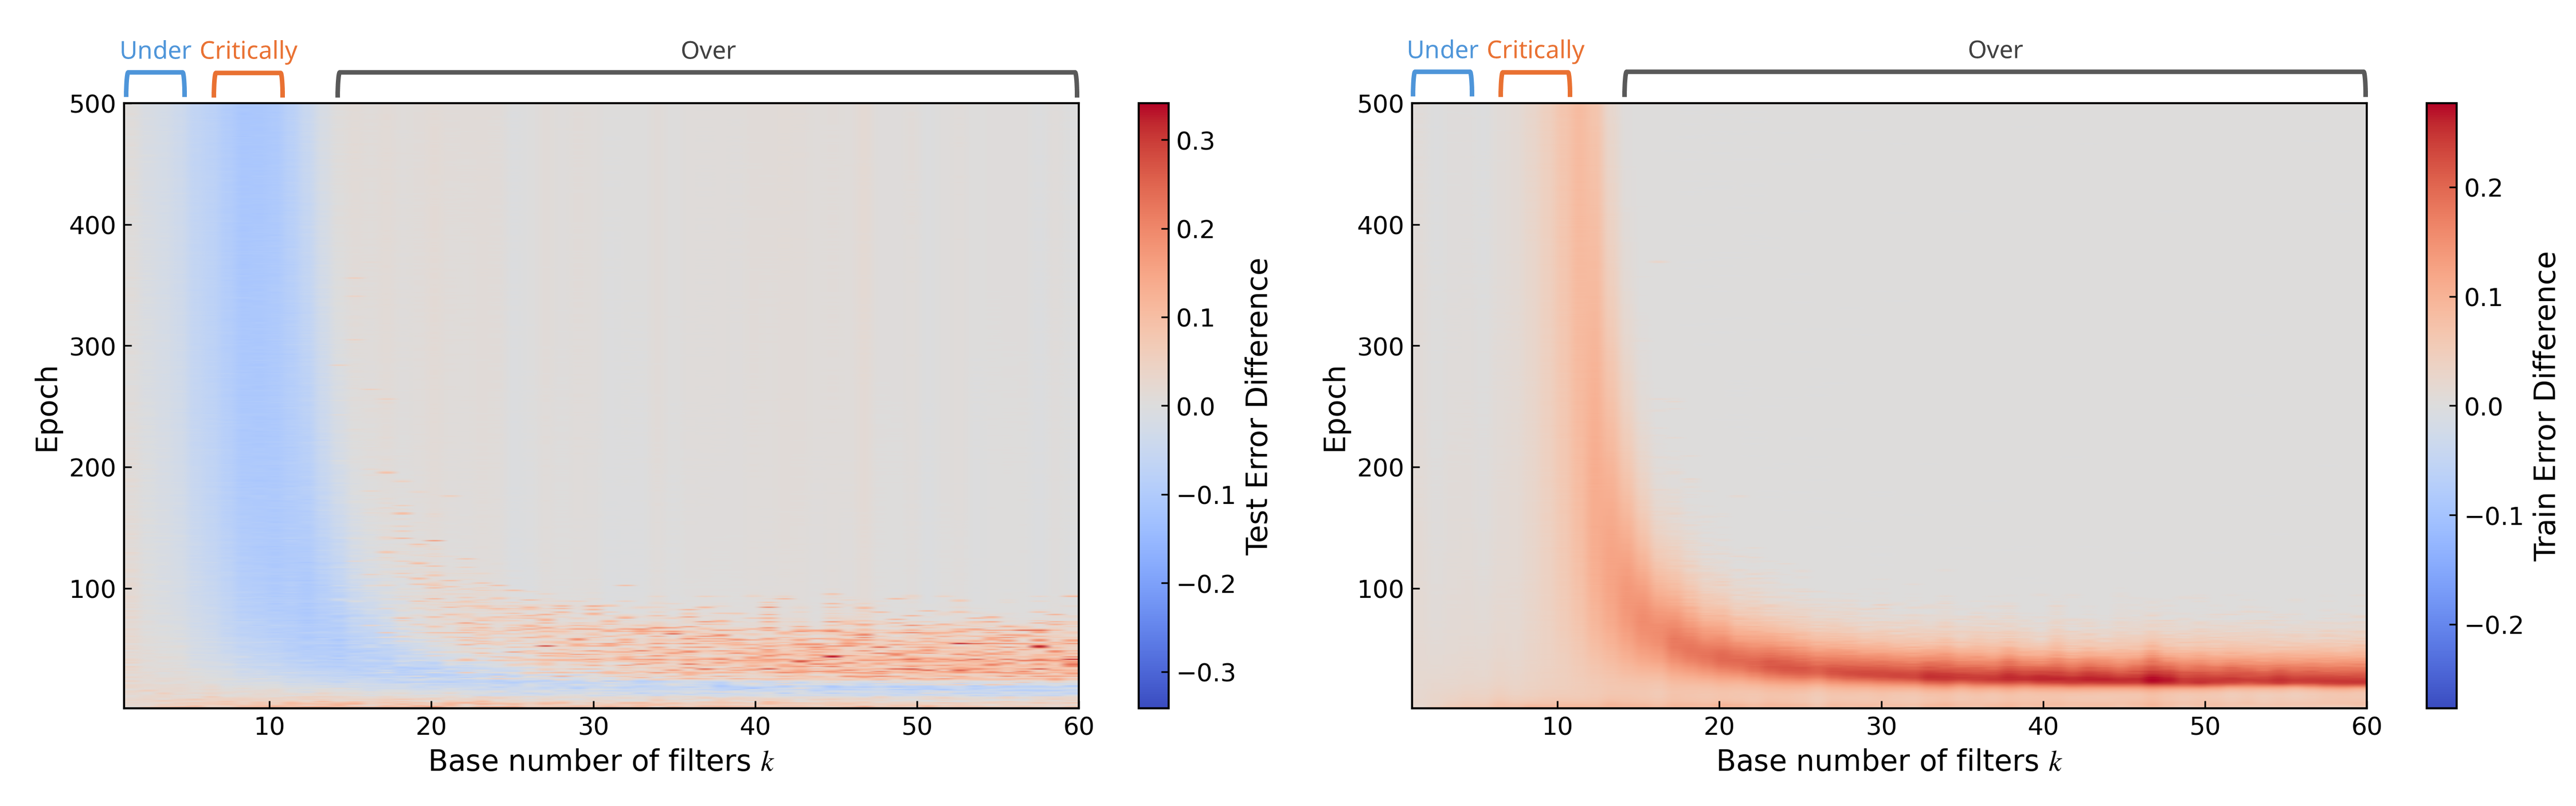
\includegraphics[width=0.8\linewidth]{fig/8_epoch_diff.png}
  \caption{}
  \label{fig:epoch_diff}
\end{figure}

The representative curves show the local behavior at selected widths.
To examine whether these differences are observed over the entire range of $k$ and epochs, Fig.~\ref{fig:epoch_diff} shows the difference heatmaps of the training and test error rates between ML and IL.
The values are computed as ML minus IL.
Thus, negative values indicate that ML achieves a lower error rate than IL, whereas positive values indicate that ML has a higher error rate than IL.

The test error difference shows that ML achieves lower test error mainly around the critical transition.
This result is consistent with the representative curves in Fig.~\ref{fig:epoch_curves}(b), where ML suppresses the increase in test error.
On the other hand, in the over-parameterized regime, the difference in test error becomes relatively small, although ML shows larger fluctuations.
The training error difference shows that ML tends to have higher training error than IL over a wide range of widths, especially around and after the critical transition.
This indicates that ML converges more slowly to the training data than IL.

\subsection{Variance Analysis Based on Bias--Variance Decomposition}

To further investigate the generalization behavior of ML and IL in double descent, we focus on variance.
Variance is an important factor in analyzing overfitting and generalization behavior.
In this experiment, we compare the variance of ML and IL using a cross-entropy-based bias--variance decomposition.

For an input sample $x$, let $\pi_i(x)$ denote the prediction distribution of the $i$-th trained model.
Following the cross-entropy-based bias--variance decomposition, the representative prediction distribution is defined as
\[
\bar{\pi}(x)
=
\mathrm{Normalize}
\left(
\exp\left(
\frac{1}{N}\sum_{i=1}^{N}\log \pi_i(x)
\right)
\right),
\]
where $N$ is the number of trained models.

The variance is then computed by averaging the KL divergence over the trained models and the test set:
\[
\mathrm{Variance}
=
\frac{1}{N}
\sum_{i=1}^{N}
\frac{1}{|\mathcal{D}_{\mathrm{test}}|}
\sum_{x \in \mathcal{D}_{\mathrm{test}}}
D_{\mathrm{KL}}
\left(
\bar{\pi}(x)\,\|\,\pi_i(x)
\right),
\]
where $\mathcal{D}_{\mathrm{test}}$ denotes the test set.

In our experiments, we set $N=5$ and use five trained models with different initial weights.
This computation is performed for each base number of filters $k$ and each training epoch.

\begin{figure}[htb]
  \centering
  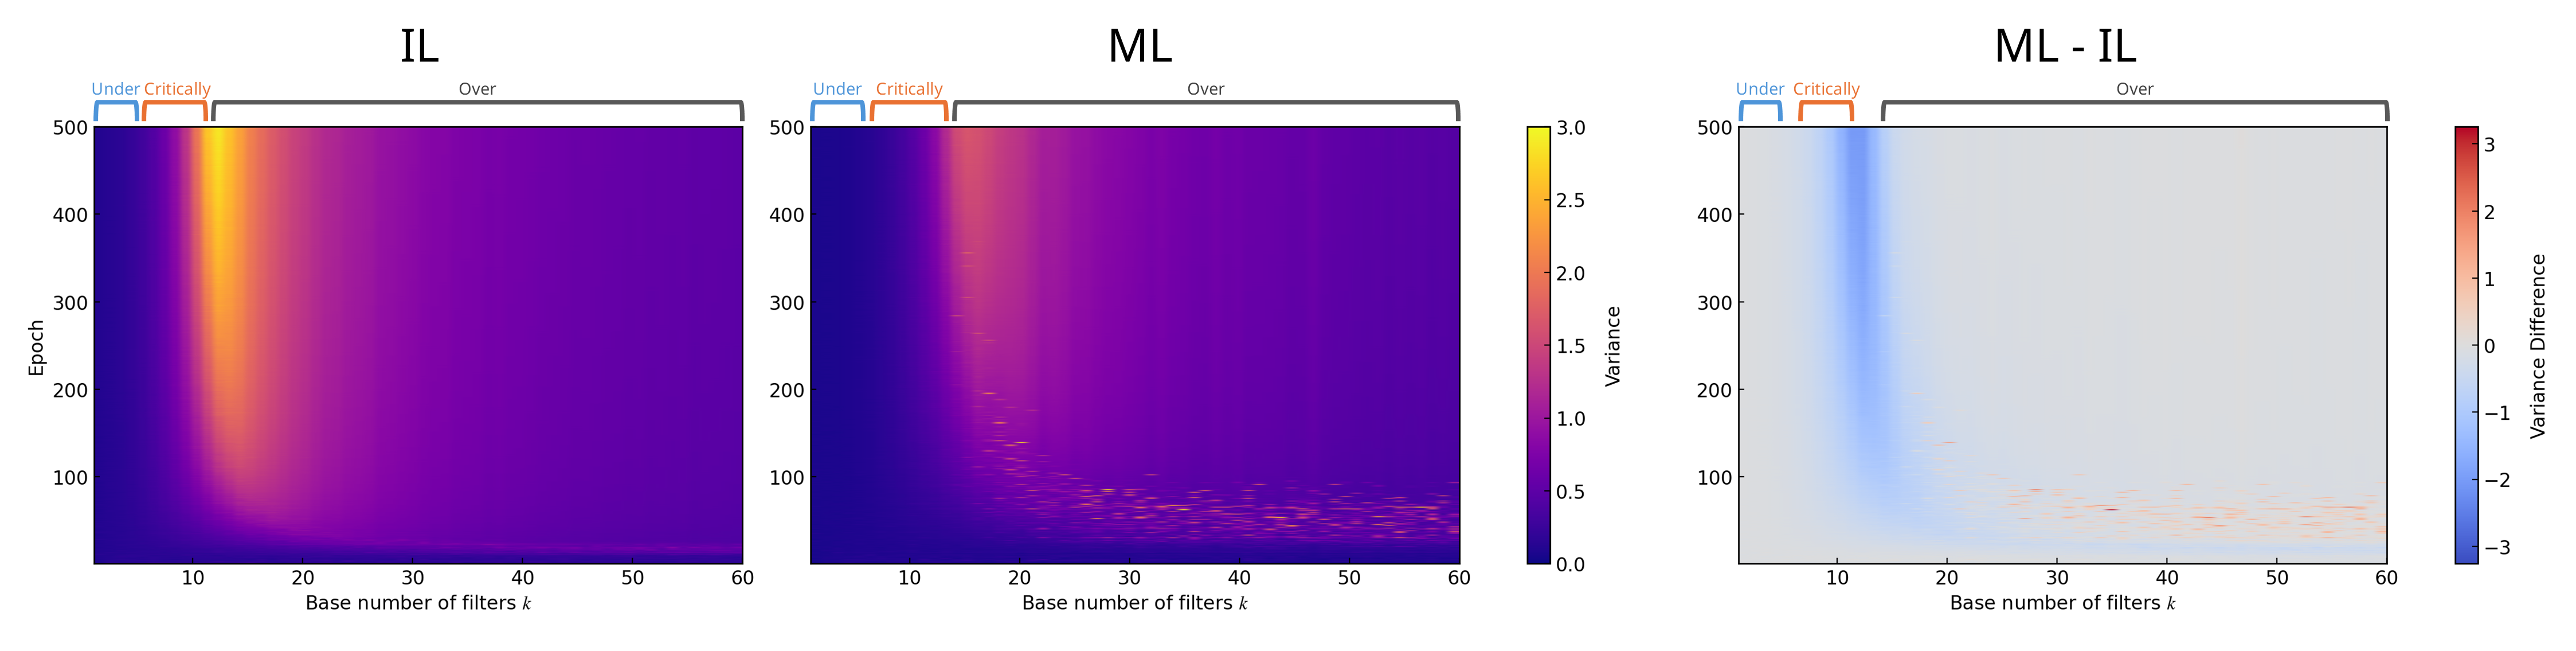
\includegraphics[width=0.8\linewidth]{fig/9_variance.png}
  \caption{Variance maps of IL, ML, and the difference between ML and IL.}
  \label{fig:variance}
\end{figure}

Figure~\ref{fig:variance} shows the variance of IL and ML as functions of the base number of filters $k$ and training epoch.
The horizontal axis represents the base number of filters $k$, the vertical axis represents the training epoch, and the color indicates the variance value.
The right panel shows the difference between ML and IL.
In the Under-parameterized regime, IL and ML show similar variance values.
In the Critical regime, the increase in variance is suppressed in ML compared with IL.
This tendency is also confirmed in the difference plot, where ML shows lower variance than IL around the Critical regime.
In the Over-parameterized regime, ML exhibits noticeable variance fluctuations in the early stage of training.

\subsection{Analysis of Solution Geometry}
The previous variance analysis indicates that ML suppresses the variability of predictions compared with IL.
To further investigate this behavior from the viewpoint of solution geometry, we analyze the sharpness and flatness of the solutions obtained by ML and IL.

We first compute the average of the top-five Hessian eigenvalues as a quantitative measure of sharpness.
Then, we visualize the loss landscape around representative filters in each regime.

\paragraph{Hessian eigenvalue analysis}
% setup
We quantitatively analyze the local curvature of the solutions obtained by ML and IL using Hessian eigenvalues.
For each trained model at each base number of filters $k$, we compute the average of the top five Hessian eigenvalues.

% results
\begin{figure}[htb]
  \centering
  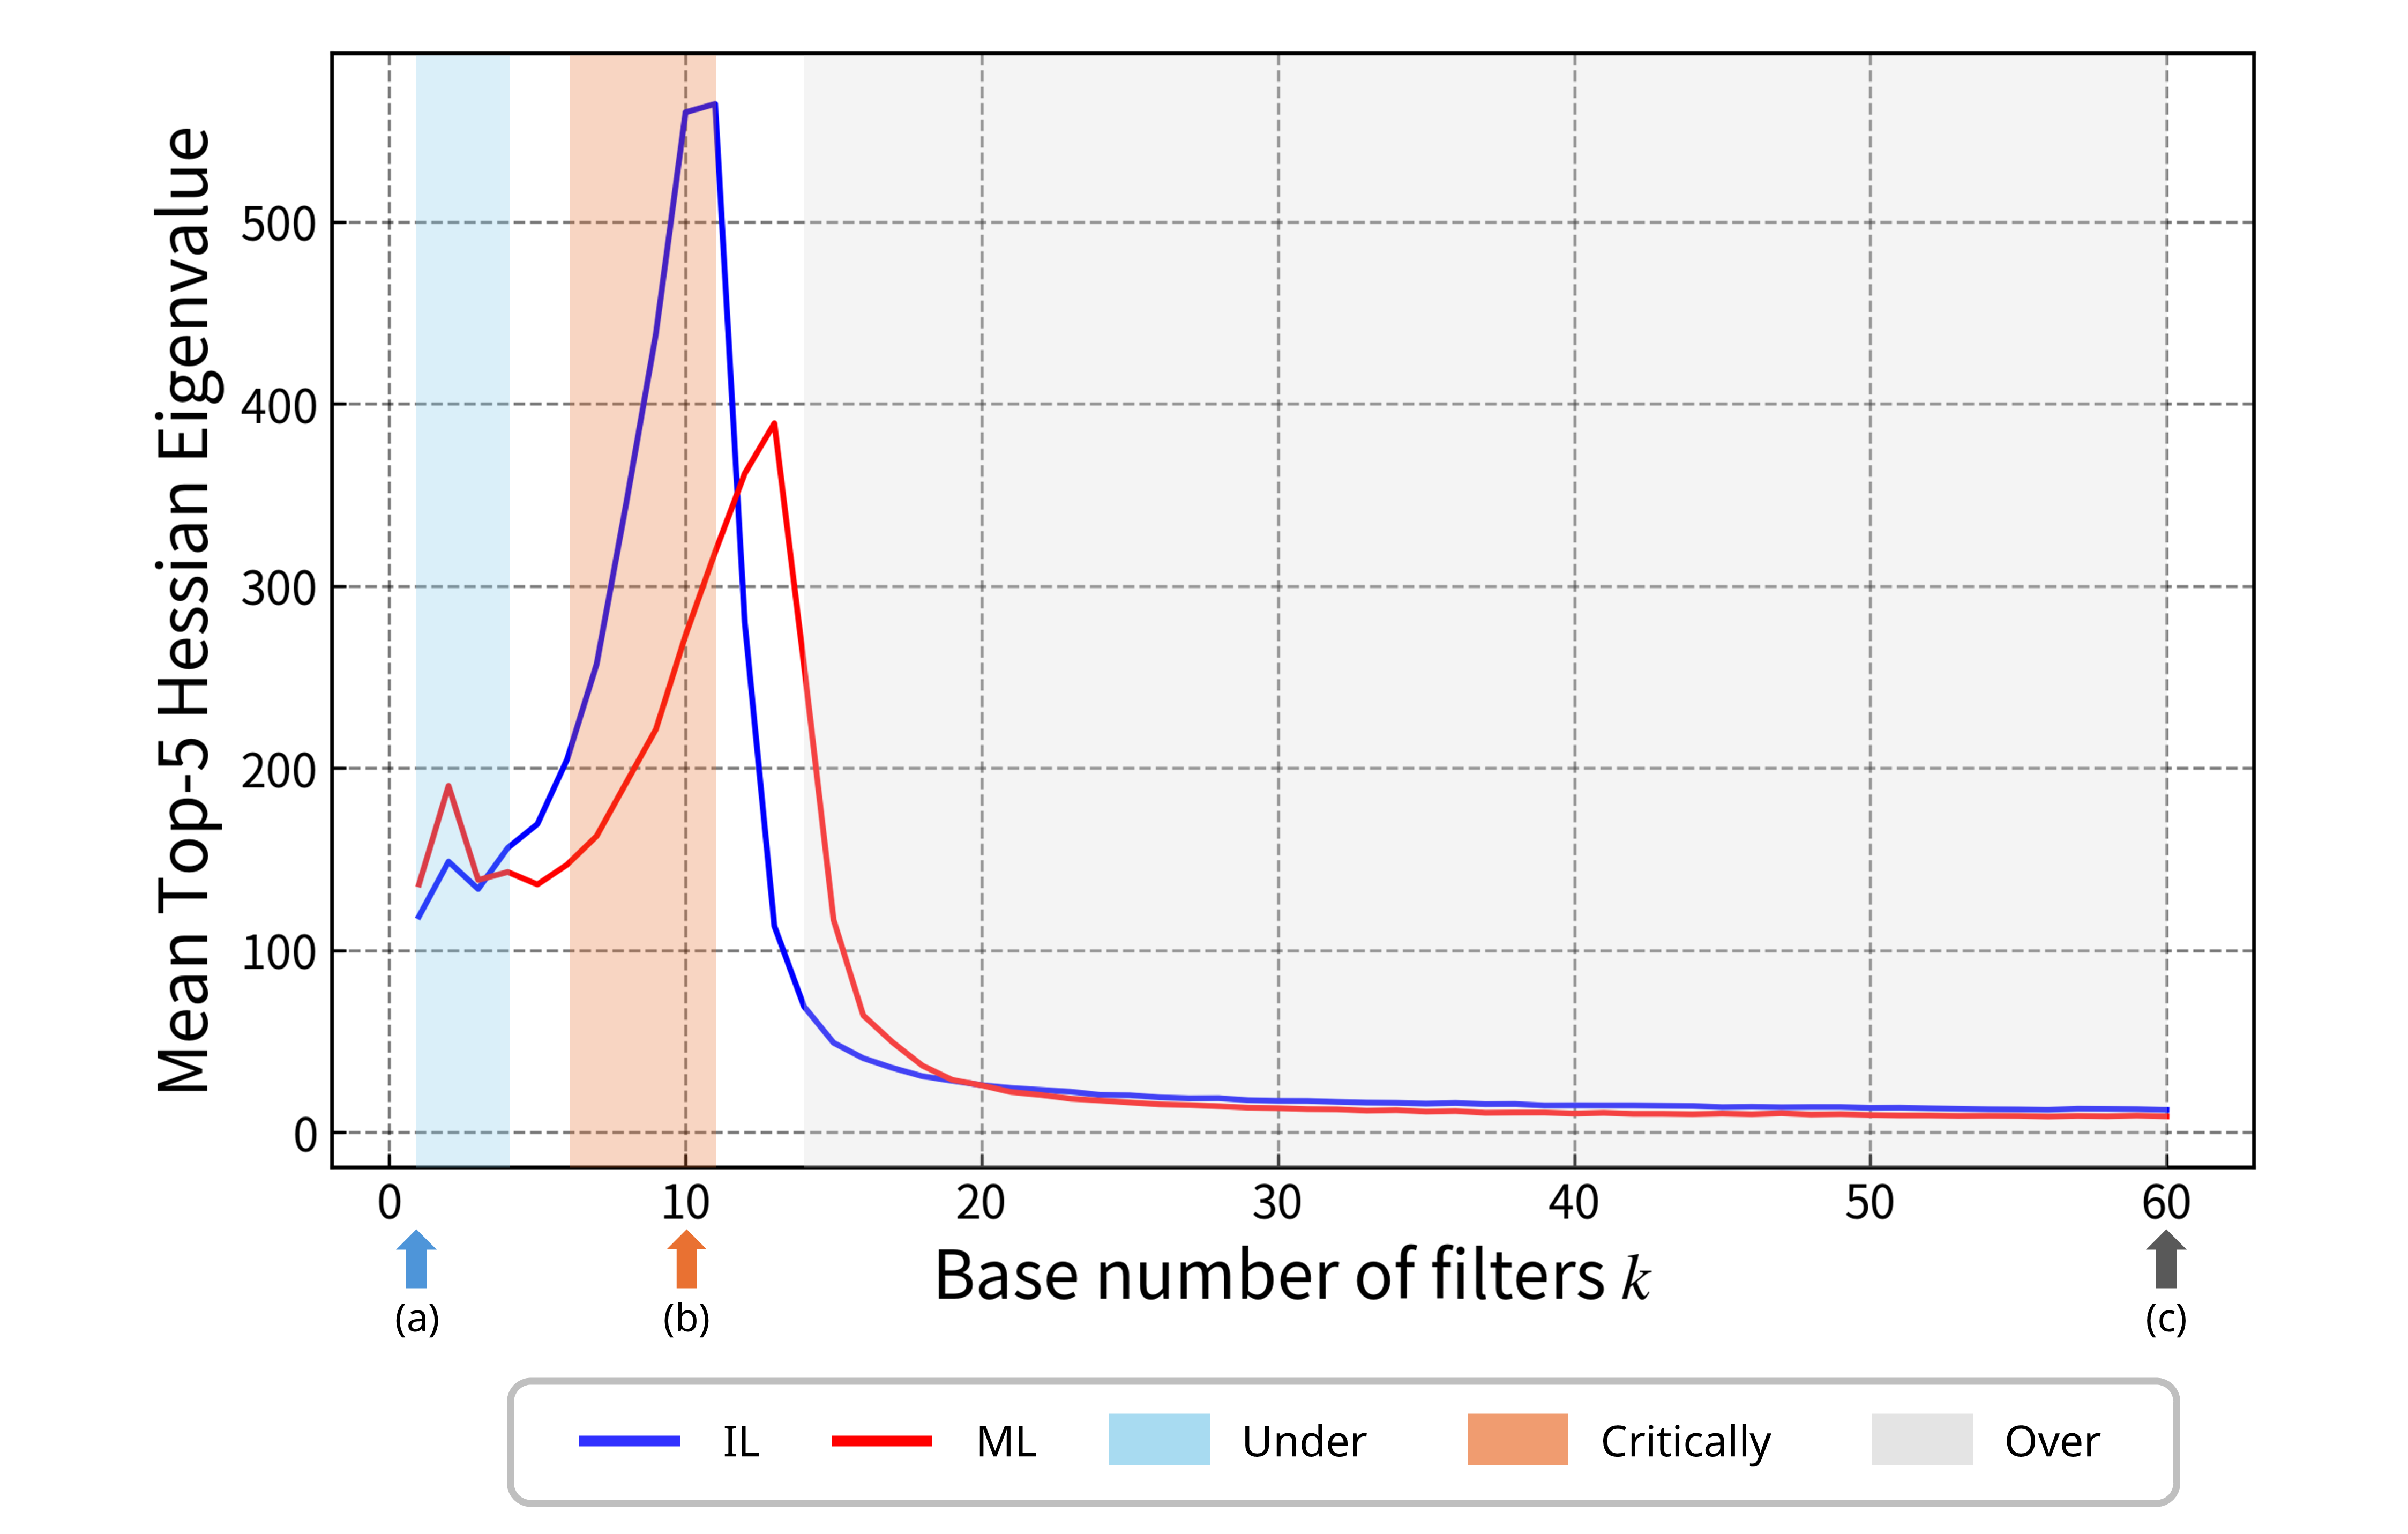
\includegraphics[width=0.8\linewidth]{fig/10_Hessian.png}
  \caption{Mean top-five Hessian eigenvalues as a function of the base number of filters $k$.}
  \label{fig:hessian}
\end{figure}

Figure~\ref{fig:hessian} shows the average of the top-five Hessian eigenvalues for IL and ML as a function of the base number of filters $k$.
The horizontal axis represents the base number of filters $k$, and the vertical axis represents the average of the top-five Hessian eigenvalues.
The blue and red curves represent IL and ML, respectively.
The shaded regions indicate the Under-parameterized, Critically-parameterized, and Over-parameterized regimes.

In the Under-parameterized regime, IL and ML show similar values, and no clear difference is observed.
In the Critically-parameterized regime, the Hessian eigenvalues of ML are much smaller than those of IL.
This result suggests that ML reaches flatter solutions than IL around the Critical regime.
In the Over-parameterized regime, the values of both methods become small, and the difference between ML and IL is also small.


\paragraph{Loss Landscape Visualization}

% setup

% results

\subsection{Error Analysis on Noisy-label and Clean-label Samples}


\section{Discussion}

\section{Conclusions}

\acknowledgments
\textcolor{blue}{(if any)}
This section should be brief and acknowledge those that have assisted in
the work or preparation of the manuscript, but who do not qualify for
authorship, as defined in the \textbf{Author Contribution} section.
Acknowledgments must be placed after the Conclusion section Declare
`\verb+\acknowledgments+' before the acknowledgment text.  To
acknowledge financial sponsors or funds, describe them into the Funding
section.

\dataavailability
\textcolor{blue}{(if any)}
Authors are encouraged to include a Data Availability in
manuscripts that report results from research data. Following
Hrynaszkiewicz et al. (2020, \url{http://doi.org/10.5334/dsj-2020-017}),
statements should include information on where the manuscript's data
can be found and hyperlinks (where applicable) to it. If research data
are not publicly available, this should be stated in this section along
with any conditions for accessing the data.
Declare  ``\verb+\dataavailability+'' before placing the Data
availability text.

\funding
\textcolor{red}{(required)}
Authors should list all funding sources for their work in the Funding
section in the following format:

This work was financially supported in part by grants
awarded to [Author(s) Initials].

Other variations are:
\begin{itemize}
\item Institution awarded the funding: [Institution name; if none, write
``None'']
\item Funder: [Funding agency name, City, Country]
\item Grant number (for each grant): [Grant number or GrantID]
\end{itemize}

If no funding was used to support the work, write ``Not applicable''
under the section heading.
Declare  ``\verb+\funding+'' before placing the Funding text.

\conflictsofinterest
\textcolor{red}{(required)}
Authors are required to declare any competing financial or other
conflicts of interest in relation to the work described. If there are no
declared interests, include a statement under the section heading
``The authors declare no competing interests.''
Declare  ``\verb+\conflictsinterest+'' before placing the
Conflict of interest text.

\authorcontribution
\textcolor{red}{(required)}
Authors are required to include a statement that specifies the
contribution of each author that follows the CRediT (Contributor Roles
Taxonomy; \url{https://credit.niso.org}) taxonomy.
One or more of the 14 CRediT taxonomy categories
should be ascribed to each author. Authors should examine the CRediT
website and include the appropriate roles for each author. An example
would be (use the actual author names in your manuscript):

\begin{tabular}{ll}
Conceptualization: & Author 1.\\
Funding acquisition: & Author 1.\\
Investigation: & Author 1, Author 2. \\
Supervision: & Author 1.\\
Visualization: & Author 3.\\
Writing--original draft: & Author 1, Author 2, Author 3.\\
Writing--review \& editing: & Author 1, Author 2.
\end{tabular}

If the work is given by authors equally, you can put
``All the authors contributed equally to the present work.''
Declare  ``\verb+\authorcontribution+'' before placing the
Author contribution text.



\ethics
\textcolor{blue}{(if any)}
Authors are required to declare they obtained and were compliant with
the relevant ethics approvals for any studies involving human or animal
subjects.
Declare  ``\verb+\ethics+'' before placing the Ethics approval and
consent to participate text.

\patientconsent
\textcolor{blue}{(if any)}
Authors are required to declare they obtained the informed consents from
patients for any relevant studies involving human subjects.
Declare  ``\verb+\patientconsent+'' before placing the Patient consent
for publication section.

\aitools
\textcolor{blue}{(if any)}
Authors are required to declare the use of Artificial intelligence tools
in the research or preparation of the manuscript. Include all relevant
details, including the name of the tool or service, a link to it, and
the purpose or reason for the use of the tool. Declare
``\verb+\aitools+'' before the Artificial intelligence tools text.

\appendix
\textcolor{blue}{(if any)}
Appendices are placed after the additional descriptions including Data
Availability, Funding, and so on, but before the References.
Declare  ``\verb+\appendix+'' before placing appendix sections.

\section{Guide for preparing multi-color display items}
Color figures can be included in NOLTA manuscripts. Authors, however,
should be reminded that some reviewers/readers may be colorblind.
Authors should consider the following suggestions when preparing figures:
\begin{enumerate}
\item Avoid using a combination of red and green. Use magenta (purple)
and green instead.
\item Do not overuse colors in the graphs but consider using different
hatching, shapes, line types (solid, dotted or dashed) or symbols for
different curves.
\item Red does not appear bright or vivid for those with colorblindness,
so avoid using red characters or symbols.
For further information, see
\url{http://jfly.iam.u-tokyo.ac.jp/color/index.html}.
\end{enumerate}

\section{NOLTA category}
The NOLTA category is used by the NOLTA Editorial Office when directing
your manuscript to the appropriate Associate Editor. Furthermore, to
help readers the category is displayed at the NOLTA websites and the
journal archives. Choose the most relevant category from the list on the
web page
\url{https://www.jstage.jst.go.jp/browse/nolta/_pubinfo/-char/en}.
The NOLTA Editorial Committee may alter the nominated subject category,
if it judges that the authors’ selection is not the optimal; this may
be done without notification to the authors.

\section{Reference format}
References should appear at the end of the manuscript, in the order in
which they are referred in the main text. See the examples in the
section elsewhere in this template for the different styles (journal
article, whole book, contributed chapter in a book, and proceedings
article).

URLs can be referenced as in \cite{web link}, below.  Articles
referenced in the manuscript should be styled as indicated in
\cite{nolta}.  If a reference has a DOI (Digital Object Identifier),
it should be indicated as in \cite{nolta, journal paper}.
An \verb+\href+ command can embed a URL of the landing page into a clickable
DOI, see this \LaTeX ~source file.
The author should confirm integrity of DOIs/URLs corresponding to the landing pages.
The styles for books and book chapters are
illustrated in \cite{book} and \cite{chapter}, respectively. The
proceedings of a conference should be referred as Proc. NOLTA'09 with
year ('09) after the conference name (NOLTA). An example is shown in
\cite{proceeding paper}.  Use a pair of square brackets to cite a
reference in the main text, for example, \cite{nolta}.  Multiple
consecutive numbered references can be cited by using a hyphen like
\cite{journal paper, book, chapter, proceeding paper}.  It is authors'
responsibility to provide correct information in the References
section.


\begin{thebibliography}{9}
\bibitem{web link} Visit \url{https:
//www.jstage.jst.go.jp/browse/nolta/_pubinfo/-char/en}
for the latest version of this template.
\bibitem{nolta} A.B. Author1, C.D. Author2, and E.F. Author3,
``Paper of NOLTA should be referenced like this,''
\textit{NOLTA},
vol.\ 1, no.\ 1, pp.\ 123--456, October 2010.
DOI:\href{https://doi.org/XX.XXXX/XXXXX}{XX.XXXX/XXXXX}
\bibitem{journal paper} A.B. Author1, C.D. Author2, and E.F. Author3,
``Title of journal paper with a comma inside the quotation marks like this,''
\textit{Journal Title in Italic},
vol.\ 12, no.\ 3, pp.\ 456--789, June 2009.
DOI:\href{https://doi.org/YY.YYYY/YYYYY}{YY.YYYY/YYYYY}
\bibitem{book}A.B. Book-Author,
\textit{Book Title in Italic without Quotation Marks},
Publisher Name, City, year.
\bibitem{chapter}A.B. Chapter-Writer, ``Title of quoted chapter''
in \textit{Book Title in Italic without Quotation Marks},
ed.\ C.D. Editor, pp.\ 123--456, Publisher Name, City, year.
\bibitem{proceeding paper}A.B. Author1, C.D. Author2,
and E.F. Author3, ``Title of
paper in proceeding,'' Proc. 6.	NOLTA'09, paper ID (if any),
pp.\ 456--789, October 2009.
\end{thebibliography}

\end{document}


